\section{Language Models - Tokenizer}\label{sec:b}

In this sections is briefly introduced the concept of \textit{token}, \textit{tokenization} and \textit{tokenizer}, how it works in a \gls{LM}, an issue when running a decentralized benchmarking, and finally a proposed solution. 

\subsection{From string to token}\label{subsec:b1}

Tokenization is the process of representing text in smaller meaningful lexical units. 
There are three popular ways to do the same, which are: 1) word tokenization, 2) subword tokenization, and 3) character tokenization. 
Word tokenization is the simplest form of tokenization, where each word is considered a token. 
Subword tokenization breaks words into subwords and treats them as tokens. 
Character tokenization considers each character as a token. 
There is a trade-off between the granularity of the tokens and the number of tokens. 
That is, while word tokenization has low granularity and high token count, character tokenization has high granularity and low token count. 
Nowadays, the most popular tokenization method is subword tokenization, which is a compromise between word and character tokenization.
It is important to note that prior to training a model, tokenizers must be trained on texts that is representative of the training set (ideally the tokenizer texts should not be part of the training set). 
With respect to the tokenizer trainin method it's worth to mention that there exist several techniques \cite{kudo_sentencepiece_2018,kudo_subword_2018,sennrich_neural_2016}

On the other hand, the tokenizer is the one in charge of carrying out the tokenization process, which consists (in a nutshell) of a dictionary that contains pairs of tokens and their numerical representation. 
For this reason, a direct relationship is established between a \gls{LM} and its tokenizer, which is crucial when evaluating the performance of a \gls{LM} since one of the main techniques for evaluating a language \gls{LM} is through the calculation of the probability of occurrence of a sequence of tokens that is conditioned by an initial sequence of tokens. 
In terms of \texttt{lm-eval-harness}\cite{biderman_lessons_2024} these two sequences are also called \texttt{context} and \texttt{continuation}, as shown in Figure \ref{fig:loglikelihood_example}.

\begin{figure}[h]
    \centering
    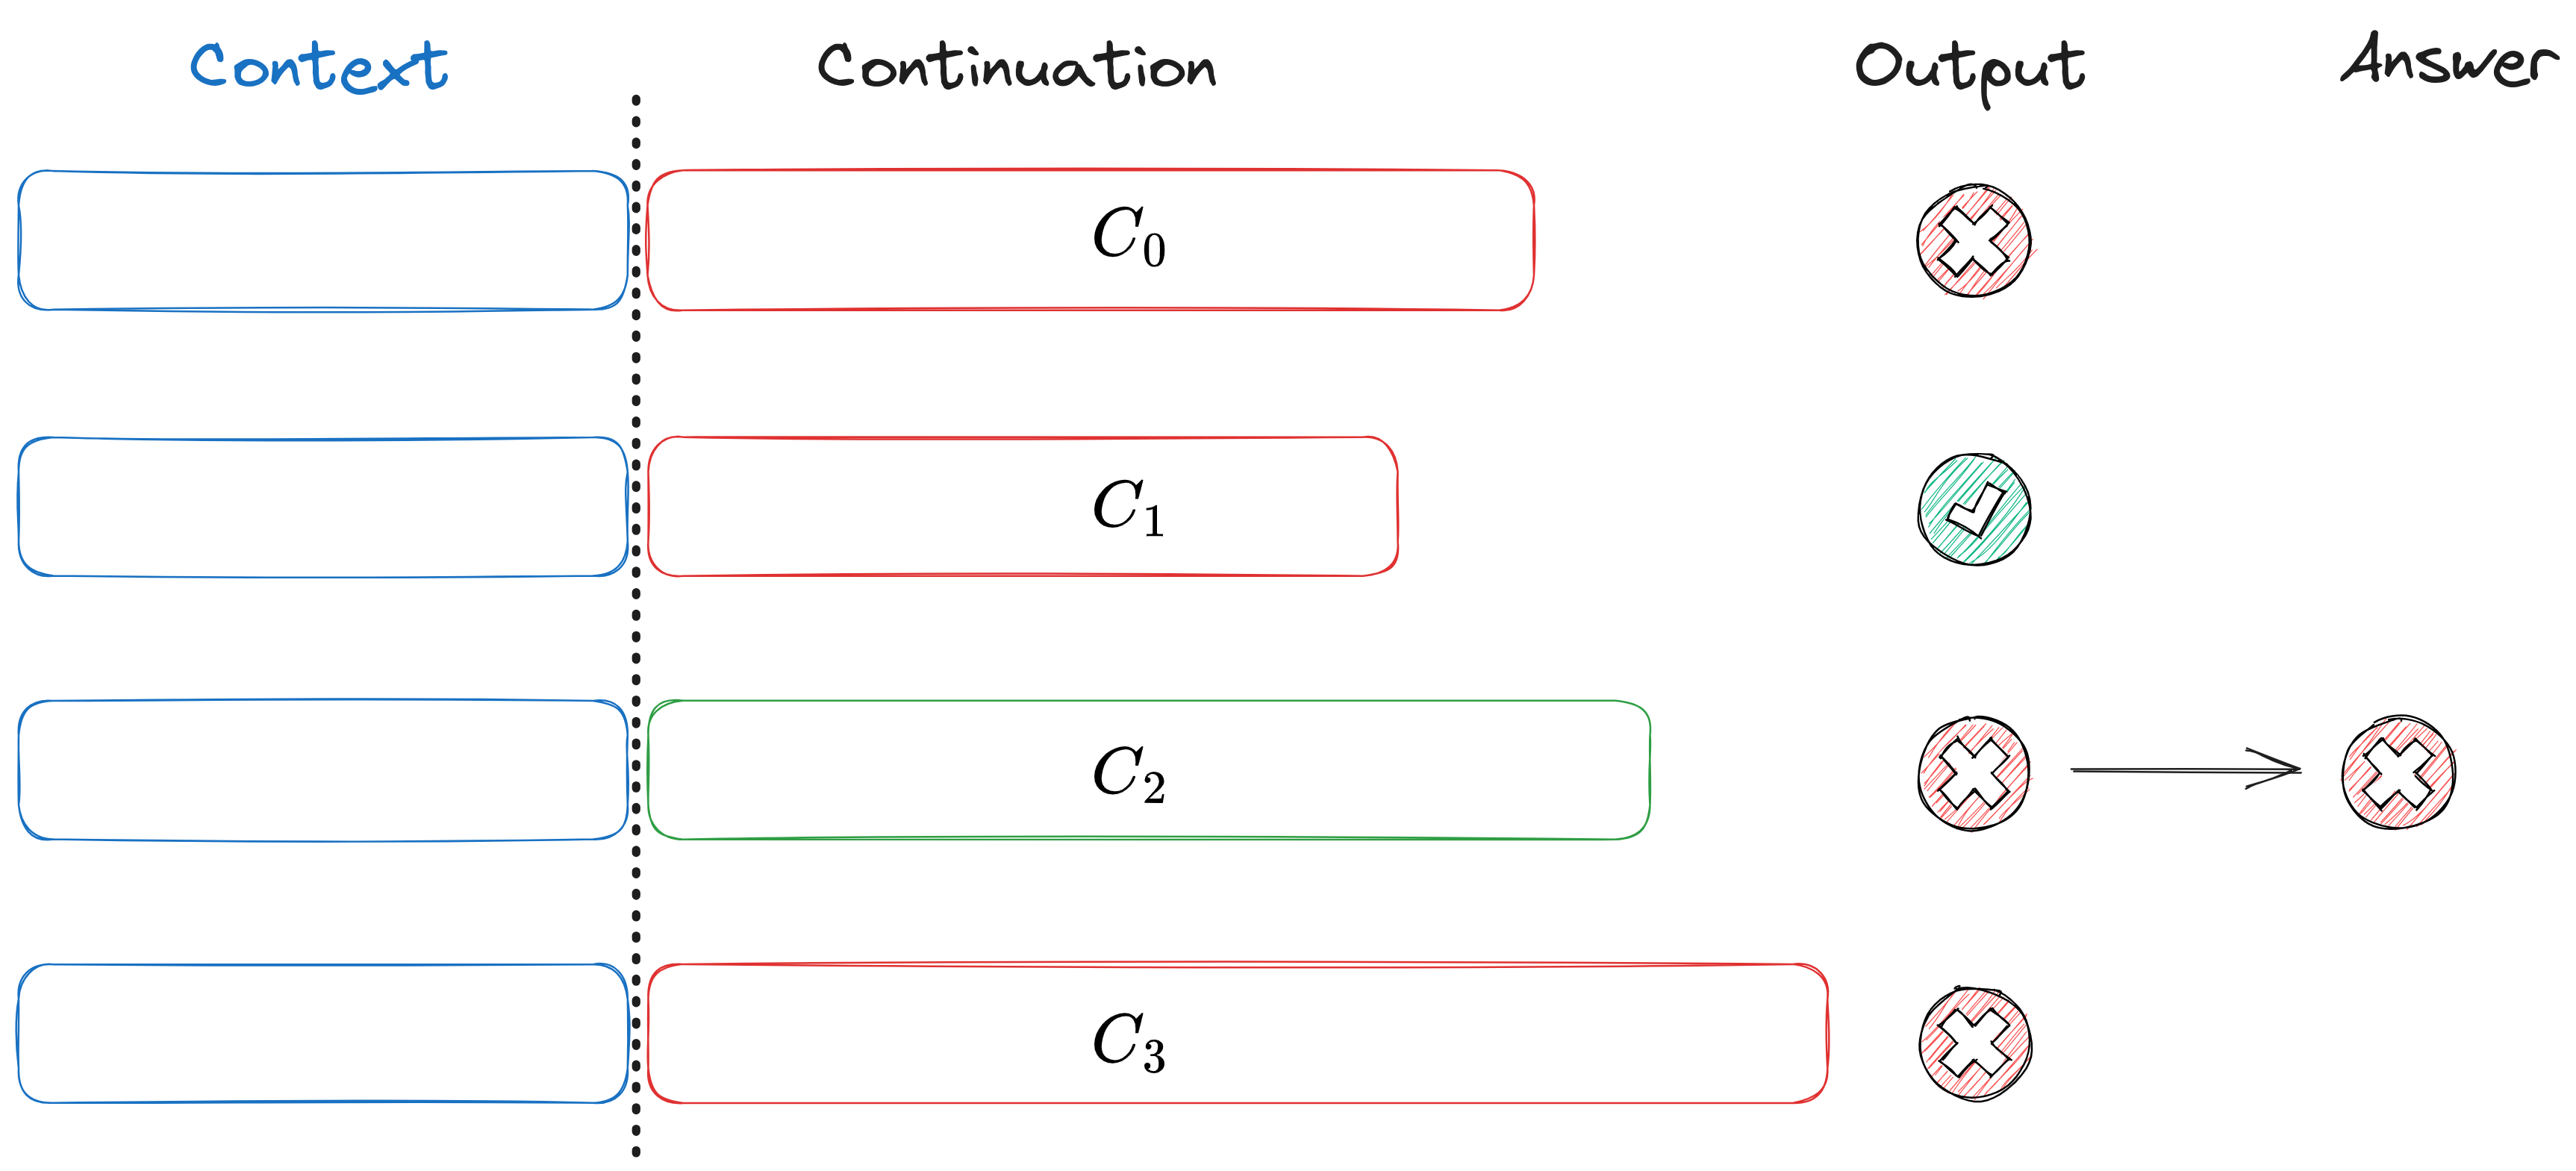
\includegraphics[width=0.8\textwidth]{img/loglikelihood_example.png}
    \caption{Example of \texttt{context} and \texttt{continuation} token sequences.}
    \label{fig:loglikelihood_example}
\end{figure}

Without going into the mathematical details, and following the Figure \ref{fig:loglikelihood_example}, the concatenation of the \texttt{context} and \texttt{continuation} tokens is sent to the language models, and from the \gls{LM} returns it can be computed the probability of occurrence of the entire phrase detailed token by token. 
The \gls{LM} is considered to respond correctly when the probability of occurrence of the correct \texttt{continuation} is the highest with respect to the other continuations. That is, in terms of the Figure \ref{fig:loglikelihood_example}, the \gls{LM} responds incorrectly, since $C_2$ should have been the \texttt{continuation} with the highest probability, but the \gls{LM} returns a higher probability for $C_1$. 

\subsection{On the lack of knowledge of the tokenizer}\label{subsec:b2}

As previously detailed, the \gls{LM} receives the concatenation of the \texttt{context} and \texttt{continuation} token sequences, and then locally separates the \texttt{context} and \texttt{continuation} probabilities. 
However, in a decentralized environment, such as that proposed by benchmarking, if you do not have access to the tokenizer, it is not possible to separate the \texttt{context} and \texttt{continuation} probabilities. 
The plain text of the concatenation of contex and \texttt{continuation} could be sent, but then we could not directly determine which part of the text belongs to the \texttt{context} and which part belongs to the continuation, thus preventing the evaluation of the model. 
Although one could try to reconstruct the \texttt{context} and \texttt{continuation} phrase from the concatenation of tokens, this is not a trivial task, since the tokenizer could have tokenized differently than the original text was tokenized \cite{biderman_lessons_2024}. 

\subsection{Proposed solution}\label{subsec:b3}

Faced with this situation, there are three other plausible solutions. 
The first solution would be to send, in addition to each complete sentence, only the \texttt{context} text. 
This would then allow us to remove those corresponding to the \texttt{context} from each of the complete sentences and continue with the evaluation of the model. 
The disadvantage of this solution is that $N+1$ calls would be made to the model, where $N$ is the number of complete sentences to evaluate, resulting in a higher cost. 
Furthermore, in the case of evaluations that contemplate the use of conversational models (such as the case of chat), this solution would not be applicable, since internally these models through its toke add special tokens to indicate the beginning and end of a message in a conversation, just as they usually have a text to condition the model's response, called system prompt. 
The second solution would be online tokenization, calling for example an endpoint \emph{tokenize}. 
This situation would face similar problems, as currently discussed in the community \footnote{\url{https://github.com/huggingface/text-generation-inference/issues/1706}}. 
The third solution would involve sending the complet tokenizer associated with an node address. 
This was detailed in two PRs \footnote{\url{https://github.com/EleutherAI/lm-evaluation-harness/pull/1794}} \footnote{\url{https://github.com/vllm-project/vllm/pull/2643}} in both the lm-eval-harness repository and the vLLM repository, popular \gls{LM} inference engine. 
The main advantage of this solution is that the issues of the first and second solutions are avoided. 
Additionally, as previously detailed, the tokenizer is tied to the model. 
Therefore we can generate a hash of the tokenizer that sends us an address, save it in a database and then verify that the hash of the tokenizer that is sent at the beginning of a session is equal to the hash stored in the database. 
If for some reason the hash does not match, it is an unequivocal indication that the \gls{LM} behind the endpoint is not the same, it has changed, therefore the previous results are not valid, metrics are eliminated from the leaderboard, and that address has to be re-evaluated. 